\documentclass[tikz,border=4pt]{standalone}
\usepackage{amsmath,amssymb}
\usepackage{mathptmx}
\usepackage{pgfplots}
\pgfplotsset{compat=1.18}
\usetikzlibrary{arrows.meta,positioning,calc,decorations.pathmorphing,backgrounds,fit,shapes.geometric}
\begin{document}
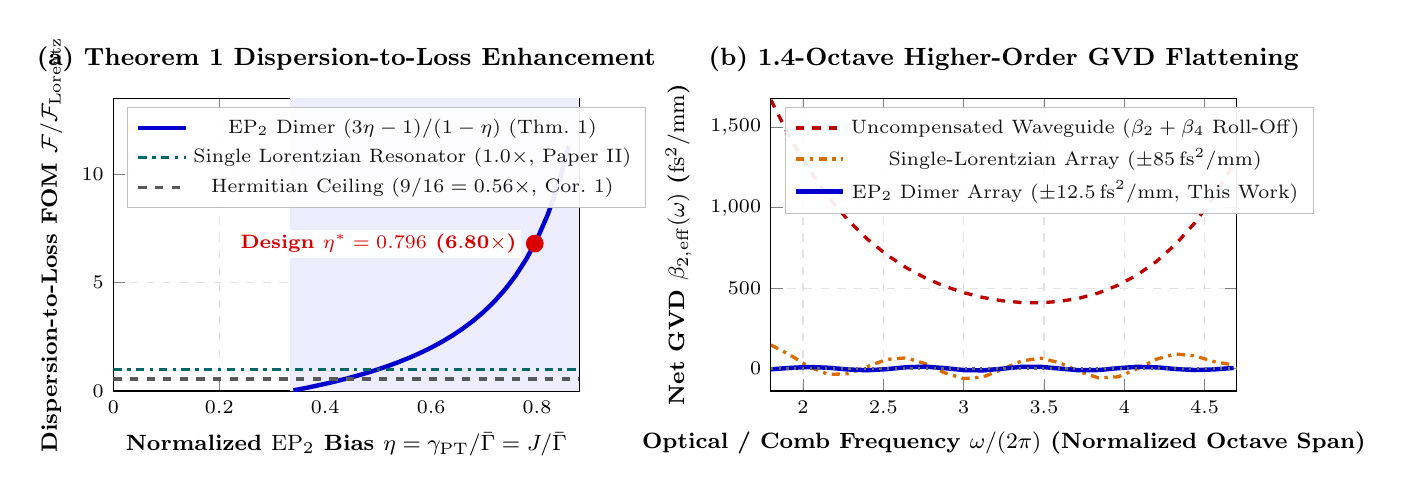
\begin{tikzpicture}[font=\small]
  % ==================== PANEL (a): Dispersion-to-Loss FOM ====================
  \begin{scope}[shift={(0,0)}]
    \begin{axis}[
      width=7.5cm,
      height=5.3cm,
      xlabel={Normalized $\mathrm{EP}_2$ Bias $\eta = \gamma_{\mathrm{PT}}/\bar{\Gamma} = J/\bar{\Gamma}$},
      ylabel={Dispersion-to-Loss FOM $\mathcal{F} / \mathcal{F}_{\mathrm{Lorentz}}$},
      xmin=0.0, xmax=0.88,
      ymin=0.0, ymax=13.5,
      grid=both,
      grid style={gray!22, dashed},
      tick label style={font=\scriptsize},
      label style={font=\footnotesize\bfseries},
      title={\textbf{(a) Theorem 1 Dispersion-to-Loss Enhancement}},
      title style={font=\small},
      legend style={at={(0.03,0.97)}, anchor=north west, font=\scriptsize, fill=white, fill opacity=0.92, draw=gray!50},
    ]
      % Shaded Anomalous Double-Pole Regime (eta > 1/3)
      \addplot[fill=blue!7, draw=none, forget plot] coordinates {(0.3333, 0.0) (0.88, 0.0) (0.88, 13.5) (0.3333, 13.5)};

      % EP2 Curve (Theorem 1)
      \addplot[blue!80!black, ultra thick] coordinates {(0.34,0.0303) (0.36,0.125) (0.38,0.22581) (0.4,0.33333) (0.42,0.44828) (0.44,0.57143) (0.46,0.7037) (0.48,0.84615) (0.5,1.0) (0.52,1.16667) (0.54,1.34783) (0.56,1.54545) (0.58,1.7619) (0.6,2.0) (0.62,2.26316) (0.64,2.55556) (0.66,2.88235) (0.68,3.25) (0.7,3.66667) (0.72,4.14286) (0.74,4.69231) (0.76,5.33333) (0.78,6.09091) (0.8,7.0) (0.82,8.11111) (0.84,9.5) (0.86,11.28571)};
      \addlegendentry{$\mathrm{EP}_2$ Dimer $(3\eta-1)/(1-\eta)$ (Thm.~1)}

      % Single Lorentzian Baseline (Paper II)
      \addplot[teal!80!black, very thick, dashdotted] coordinates {(0.0, 1.0) (0.88, 1.0)};
      \addlegendentry{Single Lorentzian Resonator ($1.0\times$, Paper~II)}

      % Passive Hermitian Anomalous Ceiling (Corollary 1: 9/16 = 0.5625)
      \addplot[gray!70!black, very thick, dashed] coordinates {(0.0, 0.5625) (0.88, 0.5625)};
      \addlegendentry{Hermitian Ceiling ($9/16 = 0.56\times$, Cor.~1)}

      % Design Point Marker at eta* = 0.7959 -> 6.80x
      \addplot[only marks, mark=*, mark size=3.0pt, red!85!black, forget plot] coordinates {(0.7959, 6.8000)};
      \node[anchor=east, font=\scriptsize\bfseries, red!85!black, fill=white, inner sep=1.5pt] at (axis cs:0.77, 6.80)
        {Design $\eta^* = 0.796$ ($\mathbf{6.80\times}$)};
    \end{axis}
  \end{scope}

  % ==================== PANEL (b): Broadband GVD Compensation ====================
  \begin{scope}[shift={(8.35,0)}]
    \begin{axis}[
      width=7.5cm,
      height=5.3cm,
      xlabel={Optical / Comb Frequency $\omega/(2\pi)$ (Normalized Octave Span)},
      ylabel={Net GVD $\beta_{2,\mathrm{eff}}(\omega)$ ($\mathrm{fs^2/mm}$)},
      xmin=1.80, xmax=4.70,
      ymin=-140, ymax=1680,
      grid=both,
      grid style={gray!22, dashed},
      tick label style={font=\scriptsize},
      label style={font=\footnotesize\bfseries},
      title={\textbf{(b) 1.4-Octave Higher-Order GVD Flattening}},
      title style={font=\small},
      legend style={at={(0.03,0.97)}, anchor=north west, font=\scriptsize, fill=white, fill opacity=0.92, draw=gray!50},
    ]
      % Bare Uncompensated Waveguide GVD
      \addplot[red!75!black, very thick, dashed] coordinates {(1.8,1670.0) (1.92,1433.27) (2.04,1232.85) (2.16,1064.11) (2.28,922.83) (2.4,805.25) (2.52,708.03) (2.64,628.29) (2.76,563.57) (2.88,511.86) (3.0,471.59) (3.12,441.63) (3.24,421.27) (3.36,410.27) (3.48,408.8) (3.6,417.5) (3.72,437.4) (3.84,470.03) (3.96,517.32) (4.08,581.64) (4.2,665.82) (4.32,773.11) (4.44,907.2) (4.56,1072.23) (4.68,1272.78)};
      \addlegendentry{Uncompensated Waveguide ($\beta_2 + \beta_4$ Roll-Off)}

      % Single-Lorentzian Compensated GVD
      \addplot[orange!85!black, very thick, dashdotted] coordinates {(1.8,146.82) (1.92,83.83) (2.04,9.41) (2.16,-36.86) (2.28,-32.33) (2.4,11.45) (2.52,56.6) (2.64,66.11) (2.76,30.43) (2.88,-25.91) (3.0,-62.56) (3.12,-53.15) (3.24,-4.78) (3.36,47.1) (3.48,64.56) (3.6,35.0) (3.72,-19.55) (3.84,-58.36) (3.96,-51.59) (4.08,-1.81) (4.2,58.28) (4.32,90.18) (4.44,78.34) (4.56,42.11) (4.68,22.21)};
      \addlegendentry{Single-Lorentzian Array ($\pm 85\,\mathrm{fs^2/mm}$)}

      % EP2 Dimer Compensated GVD
      \addplot[blue!80!black, ultra thick] coordinates {(1.8,-4.93) (1.92,3.99) (2.04,9.46) (2.16,4.73) (2.28,-5.88) (2.4,-10.82) (2.52,-3.98) (2.64,7.79) (2.76,11.56) (2.88,2.72) (3.0,-9.41) (3.12,-11.53) (3.24,-1.14) (3.36,10.5) (3.48,10.73) (3.6,-0.53) (3.72,-10.87) (3.84,-9.27) (3.96,2.01) (4.08,10.47) (4.2,7.4) (4.32,-3.09) (4.44,-9.42) (4.56,-5.43) (4.68,3.66)};
      \addlegendentry{$\mathrm{EP}_2$ Dimer Array ($\pm 12.5\,\mathrm{fs^2/mm}$, This Work)}

      % Zero-GVD reference line
      \draw[dotted, black!60, thick] (axis cs:1.80, 0.0) -- (axis cs:4.70, 0.0);
    \end{axis}
  \end{scope}
\end{tikzpicture}
\end{document}
